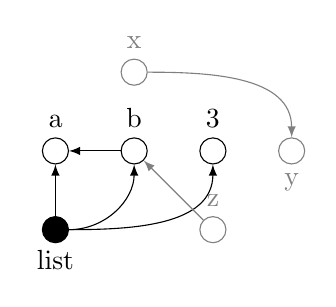
\begin{tikzpicture}[node distance=1cm]
  \node [draw,circle,label={a}]    (a)              {};

  \node [draw,circle,label={b}]    (b) [right of=a] {};
  \draw[-latex] (b.west) -- (a.east);

  \node [draw,circle,label={3}]    (3) [right of=b] {};

  \node [draw,circle,fill,label={[label distance=-0.8cm]:list}] (l) [below of=a] {};
  \draw[-latex] (l.north) -- (a.south);
  \draw[-latex] (l.east) to [out=0,in=270] (b.south);
  \draw[-latex] (l.east) to [out=0,in=270] (3.south);


  \node [draw,circle,color=gray,label={[color=gray]x}] (x) [above of=b] {};
  \node [draw,circle,color=gray,label={[color=gray,label distance=-0.8cm]y}] (y) [right of=3] {};
  \draw[-latex,color=gray] (x.east) to [out=0,in=90] (y.north);
  \node [draw,circle,color=gray,label={[color=gray]z}] (z) [below of=3] {};
  \draw[-latex,color=gray] (z) -- (b);
\end{tikzpicture}
